\section{Method}

\subsection{Task Formulation}

Given an RGB image $I$, a free-form instruction $q$, and a set of visible Molmo candidates
\begin{equation}
\mathcal{C}=\{c_i=(i,p_i)\}_{i=1}^{K},
\end{equation}
where $i$ is a visible numeric mark and $p_i=(x_i,y_i)$ is its image point, the system predicts the object ID $i^{*}$ that should be grasped now and a corresponding mask $\hat{M}$. The first-grasp object may be the requested target or a visible blocker whose removal is required before the target can be grasped.

We evaluate two binary outcomes. Reasoning success rate (RSR) measures whether the selected ID maps to an acceptable first-grasp instance. Segmentation success rate (SSR) measures whether $\hat{M}$ reaches IoU $\geq 0.5$ with an acceptable ground-truth first-grasp mask. Ground-truth instance IDs and masks are used only by the scorer after prediction.

\subsection{Inference Evidence Boundary}

EGHC uses only deployment-available inference evidence. The evidence packet contains Molmo candidate IDs and points, predicted masks or boxes, predicted spatial relations, parser validity flags, and route-specific consistency signals. It does not contain ground-truth semantic labels, ground-truth instance masks, benchmark difficulty labels, or Molmo-to-ground-truth mappings.

This boundary is important because earlier v10/S1 diagnostic experiments used annotation-derived semantic and geometric features. Those runs remain useful for measuring oracle headroom, but they are not treated as deployable method results. EGHC3\_v3 is the frozen main method because its manifest records \texttt{feature\_source=deployable\_predicted}, \texttt{uses\_gt\_features=false}, and \texttt{uses\_benchmark\_difficulty=false}.

\subsection{Evidence-Gated Hierarchical Consensus Routing}

The routing stage converts evidence into one of three decision modes:
\begin{itemize}
    \item \texttt{direct}: the target appears visible and unobstructed, so the target itself should be grasped.
    \item \texttt{target\_first}: the target must be resolved before deciding whether a blocker is needed.
    \item \texttt{blocker\_first}: evidence indicates that a visible object should be removed before the target can be grasped.
\end{itemize}

The gate is conservative. A direct decision requires a valid visible target ID and no credible blocker or ambiguity evidence. A blocker-first decision requires physical evidence such as contact, coverage, on-top, overlap, or a strong visibility conflict; image-space proximity alone is insufficient. Ambiguous or inconsistent evidence falls back to target-first reasoning rather than forcing a blocker.

Hierarchical consensus is then used to stabilize the final route and first-grasp ID. The first stage proposes a route from the evidence packet. The second stage performs route-specific planning using the selected protocol. A lightweight repair or adjudication call is triggered only when the selected ID is invalid, the direct route conflicts with blocker evidence, or the target/blocker decision is internally inconsistent. This keeps the decision auditable: every final prediction can be traced to the evidence fields and guard reasons that allowed or rejected a route.

\subsection{Route-Specific First-Grasp Planning}

All routes return a parser-compatible structured decision:
\begin{verbatim}
{
  "target_resolution": {...},
  "blocker_evidence": [...],
  "first_grasp_decision": {
    "object_id": 3,
    "action": "pick_target",
    "mask_query": "red box",
    "ranked_candidates": [3, 5, 2]
  }
}
\end{verbatim}

The direct route is optimized for visible, unblocked targets. The target-first route separates target identity from the immediate first-grasp object, which reduces the chance that the model confuses the requested object with a blocker. The blocker-first route requires a visible and immediately graspable blocker and rejects unsupported nearby distractors. Ranked candidates are retained for mask repair, but the primary RSR decision remains the selected first-grasp ID.

\subsection{Point- and Evidence-Constrained Mask Repair}

After first-grasp planning, the selected visual phrase is passed to the segmentation backend. The repair stage is deterministic rather than learned or tuned. Its dominant constraint is point consistency with the selected Molmo candidate:
\begin{equation}
\mathcal{M}_{p}=\{M\in\mathcal{M}:p_{i^{*}}\in M\}.
\end{equation}
If at least one returned mask contains the selected point, EGHC chooses the smallest containing mask after filtering masks whose normalized area exceeds 0.65; if all containing masks exceed this threshold, it still chooses the smallest containing mask rather than switching to a different instance. If no returned mask contains the point, the stage records a point-consistency failure and tries simplified noun phrases and ranked fallback candidates. Only when no point-consistent retry succeeds does it fall back to the closest available mask. When no Molmo point is available, the system selects the highest-logit LangSAM mask. Thus, point consistency acts as a hard priority, normalized area is a fixed plausibility filter, and segmentation confidence is used only in the no-point fallback case.

\begin{figure}[t]
    \centering
    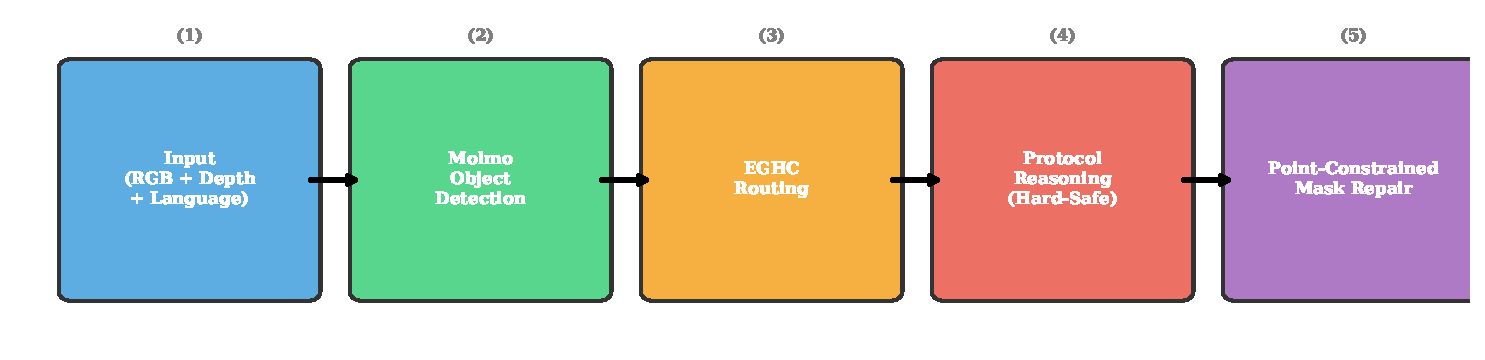
\includegraphics[width=\columnwidth]{figures/system_overview.pdf}
    \caption{EGHC overview. Molmo candidates and predicted evidence feed an evidence gate, hierarchical route consensus, route-specific first-grasp planning, and point-constrained mask repair. Ground-truth masks and difficulty labels are isolated to the scorer and are not inference inputs.}
    \label{fig:overview}
\end{figure}

\begin{figure}[t]
    \centering
    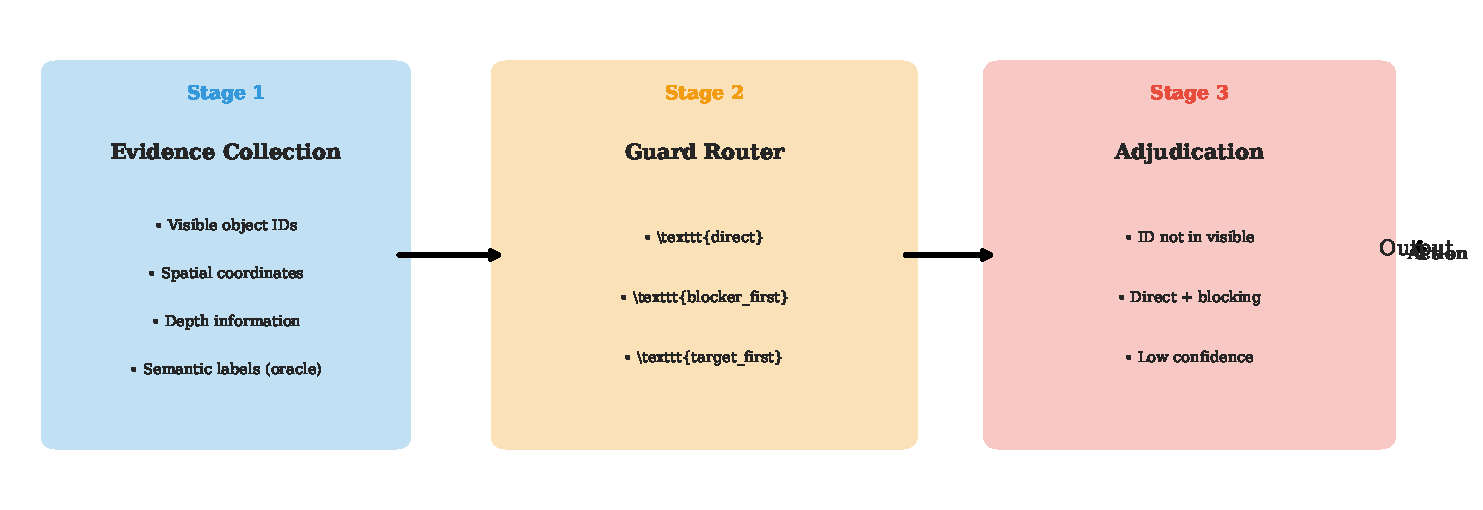
\includegraphics[width=\columnwidth]{figures/eghc_architecture.pdf}
    \caption{Evidence-Gated Hierarchical Consensus Routing. Direct decisions require strong target evidence and no blocker conflict; ambiguous evidence falls back to target-first reasoning; blocker-first decisions require explicit physical blocker evidence.}
    \label{fig:eghc}
\end{figure}
